\documentclass[a4paper,12pt]{report}
\usepackage[utf8]{inputenc}
\usepackage[francais]{babel}
\usepackage{fancyhdr}
\usepackage{graphicx}
\usepackage{tikz}
\usetikzlibrary{calc}
\usepackage{listings}
\usepackage{xcolor}
\definecolor{grey}{rgb}{0.9,0.9,0.9}
\usepackage{titlesec}
\usepackage{verbatim}
\usepackage{listings}
\usepackage{textcomp}
\usepackage{hyperref}
\usepackage{ amssymb }


\frenchbsetup{StandardLists=true}
\newcommand{\marge}{18mm}
\usepackage[left=\marge,right=\marge,top=\marge,bottom=\marge]{geometry}
\pagestyle{fancy}
\setlength{\headheight}{14pt}
\chead{
  \textbf{Binôme :} Douaille Erwan \& Yanis Nait Abdelaziz
  \hspace{2em}
  \textbf{Groupe :} M1 Info TI}
\renewcommand{\headrulewidth}{1pt}
\linespread{1}
\setlength{\columnseprule}{0.2pt}


\begin{document}



\makeatletter
\begin{titlepage}
\centering
\vspace{-10em}
{\LARGE \textbf{\textsc{Rapport de Projet RVI}}}\\
\vspace{3em}

\includegraphics[scale=0.6]{image/thalassa.png}\\
\vspace{3em}
{\LARGE \textsc{Projet Thalassa: simulation de plongée sous-marine}}\\

\vspace{8em}
Par\\
\vspace{1em}
{\LARGE \@author}\\

\vspace{2em}



\begin{tikzpicture}[remember picture,overlay]

\node [below left,xshift=-1cm, yshift=4cm] at (current page.south east){
\includegraphics[scale=0.6]{image/ustl1.png}};

\end{tikzpicture}
\end{titlepage}
\makeatother

\sloppy

\setcounter{page}{1} 
\newpage

%%%%%%%%%%%%%%%%%%%%%%%%%%%%%%%%%%%%%%%%%% INTRO
%%%%%%%%%%%%%%%%%%%%%%%%%%%%%%%%%%%%%%%%%%%%%%%%%
%%%%%%%%%%%%%%%%%%%%%%%%%%%%%%%%%%%%%%%%%%%%%%%%%
\section*{Introduction}
Dans ce TP, nous allons utiliser les composantes des pixels d'une image afin de réaliser des opérations telles que le sous-échantillonage , le sur-échantillonage ou la quantification. Ces composantes peuvent prendre soit la valeur du pixel en RGB soit en niveau de gris. Un pixel d'une image couleur est composé de 3 valeurs numériques (Rouge,Vert,Bleu) tandis qu'un pixel d'une image en niveau de gris n'est composée que d'une seule valeur numérique (Gris).

%%%%%%%%%%%%%%%%%%%%%%%%%%%%%%%%%%%%%%%%%% PART 1
%%%%%%%%%%%%%%%%%%%%%%%%%%%%%%%%%%%%%%%%%%%%%%%%%
%%%%%%%%%%%%%%%%%%%%%%%%%%%%%%%%%%%%%%%%%%%%%%%%%
\section*{Composantes d'une image couleur}

\subsection*{Quelle sont les dimensions de la variable utilisée pour stocker l'image et que représentent-t-elles?}

\noindent Avec la fonction size, on obtient 3 paramètres, 600 qui définit la hauteur, 800 la largeur et 3 qui indique le nombre de composantes couleurs. L'image est donc stockée dans une matrice à 3 dimensions.

\subsection*{Séparer les composantes rouge, verte et bleue de cette image afin de les afficher tout d'abord sous la forme de trois images en niveaux de gris}

\begin{figure}[!ht]
	\center
	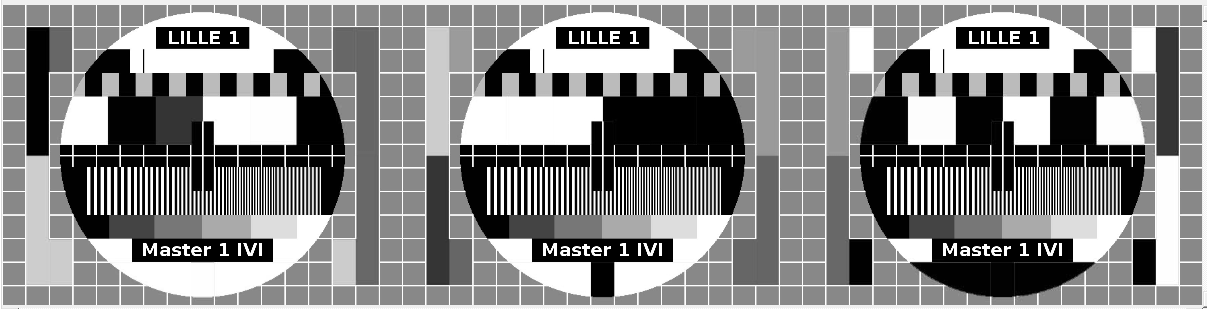
\includegraphics[scale=0.4]{image/p11.png}
\end{figure}

\subsection*{sous la forme de pseudo-images couleur}

\begin{figure}[!ht]
	\center
	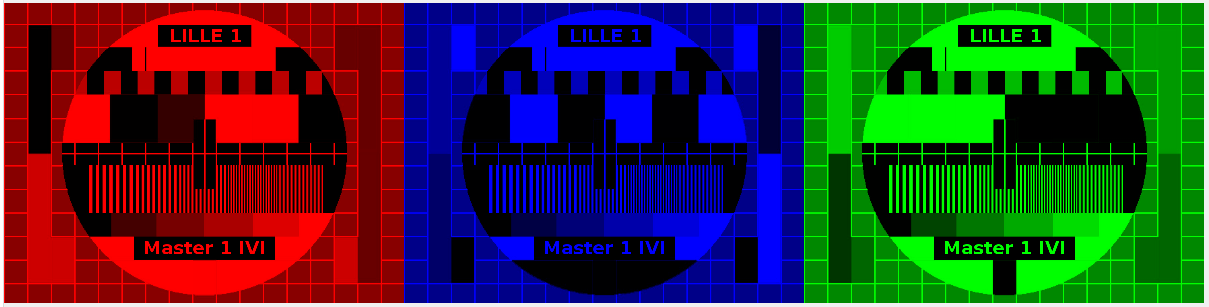
\includegraphics[scale=0.4]{image/p12.png}
	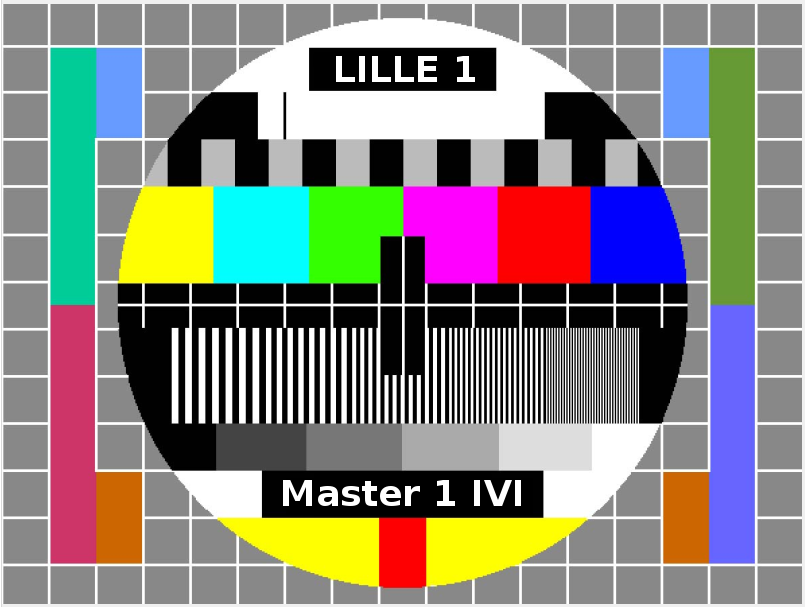
\includegraphics[scale=0.4]{image/p13.png}
\end{figure}

\noindent On constate que si on additionne les 3 images on obtient bien l'image d'origine.

\newpage

%%%%%%%%%%%%%%%%%%%%%%%%%%%%%%%%%%%%%%%%%% PART 2
%%%%%%%%%%%%%%%%%%%%%%%%%%%%%%%%%%%%%%%%%%%%%%%%%
%%%%%%%%%%%%%%%%%%%%%%%%%%%%%%%%%%%%%%%%%%%%%%%%%
\section*{Sur et sous-échantillonnage}

\subsection*{En considérant que l'image de mire utilisée précédemment a été acquise avec une résolution de 72 pixels/pouce selon les deux directions, déterminer les dimensions du support initial de l'image}

\noindent Pour obtenir les dimensions du support initial il suffit de faire 600/72 et 800/72. On obtient un support de $\sim$8,33 pouces  de hauteur et $\sim$11,11
pouces de largeur.
\subsection*{Écrire une fonction qui permet, en utilisant les données numériques d'une image (à une composante), de simuler un échantillonnage avec un capteur dont les résolutions horizontale et verticale sont n fois plus petites que celles du capteur initial (avec n entier)}

\begin{lstlisting}
function im = sousEchantillon(img,n)
    img = im2double(img);
    colonne = size(img,1)/n
    ligne = size(img,2)/n
    im = zeros(colonne,ligne)
    for i = 1 : colonne
        for j = 1 : ligne
                for n1 = 1 : n
                    for n2 = 1 : n
                        x = i*n + n1-n
                        y = j*n + n2-n
                        im(i,j) = im(i,j) + img(x,y);
                    end
                end
                im(i,j) = im(i,j) / (n*n);
        end
    end
endfunction
\end{lstlisting}

\begin{figure}[!ht]
	\center
	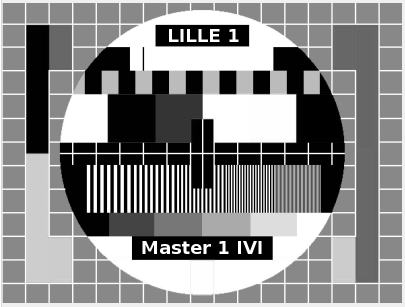
\includegraphics[scale=0.5]{image/p22.png}
\end{figure}

\noindent Le sous-échantillonage consiste à parcourir l'image, et pour le pixel concerné faire une moyenne des n*n pixels voisins pour créer un unique pixel dans l'image de destination. Avec le sous-échantillonage on perd en précision/détail de l'image.

\subsection*{Écrire une fonction qui permet, en utilisant les données numériques d'une image (à une composante), de simuler un échantillonnage avec un capteur dont les résolutions horizontale et verticale sont n fois plus grandes que celles du capteur initial (avec n entier). On appelle ce processus sur-échantillonnage de l'image}

\begin{lstlisting}
function im = surEchantillon(img,n)
  img = im2double(img);
  colonne = size(img,1)*n
  ligne = size(img,2)*n
  im = zeros(colonne,ligne)
  for i = 1 : colonne/n
      for j = 1 : ligne/n
          for n1 = 1 : n
              for n2 = 1 : n
                  x = i*n + n1-n
                  y = j*n + n2-n
                  im(x,y) = img(i,j);
              end
          end
      end
  end
endfunction
\end{lstlisting}

\begin{figure}[!ht]
	\center
	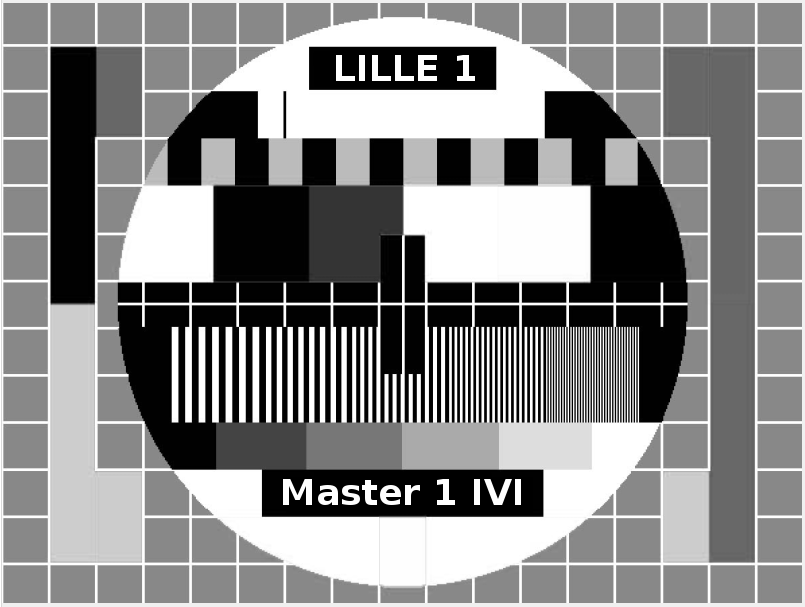
\includegraphics[scale=0.6]{image/p23.png}
\end{figure}

\noindent Le sur-échantillonage consiste à faire l'inverse du sous-échantillonage. Pour chaque pixel de l'image source, on crée n*n pixels dans l'image destination.

\subsection*{ppliquer successivement l'opération de sous-échantillonnage sur l'image initiale, puis l'opération de sur-échantillonnage sur l'image sous-échantillonnée. Que constate-t-on?}

\begin{figure}[!ht]
	\center
	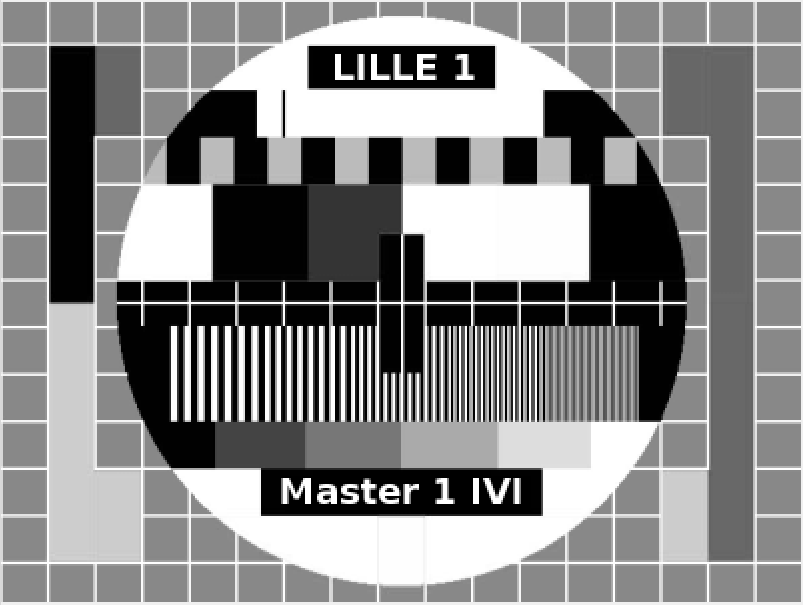
\includegraphics[scale=0.6]{image/p24.png}
\end{figure}

\noindent On constate clairement qu'un flou est apparu. Cela paraît logique puisque dans un premier temps on perd de l'information et donc de la précision à cause du sous-échantillonage et ensuite on sur-échantillone cette même image. 

C'est visible sur le contour des lettres, dans les éléments précis comme les lignes.


\newpage
%%%%%%%%%%%%%%%%%%%%%%%%%%%%%%%%%%%%%%%%%% PART 3
%%%%%%%%%%%%%%%%%%%%%%%%%%%%%%%%%%%%%%%%%%%%%%%%%
%%%%%%%%%%%%%%%%%%%%%%%%%%%%%%%%%%%%%%%%%%%%%%%%%
\section*{Quantification}

\subsection*{Écrire une fonction qui simule la quantification des valeurs des pixels d'une image}

\begin{lstlisting}
function im = quantification(img,n)
    quantificateur = 2^n
    im = img ./(256/quantificateur)
    im = im.*(256/quantificateur)
endfunction
\end{lstlisting}

\subsection*{Utiliser cette fonction pour calculer les images qui seraient obtenues avec une quantification sur 6 bits, 4 bits et enfin 1 bit de la composante verte de l'image de mire}

\begin{figure}[!ht]
	\center
	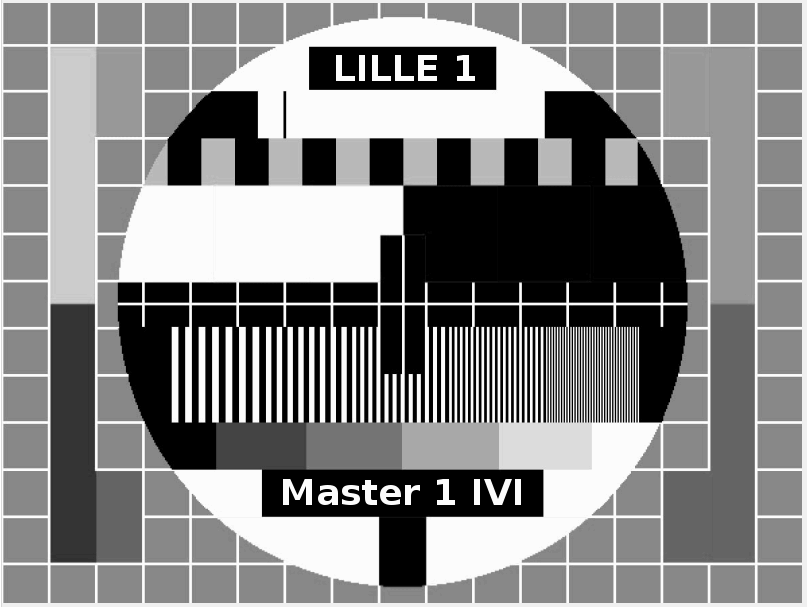
\includegraphics[scale=0.3]{image/p321.png}
	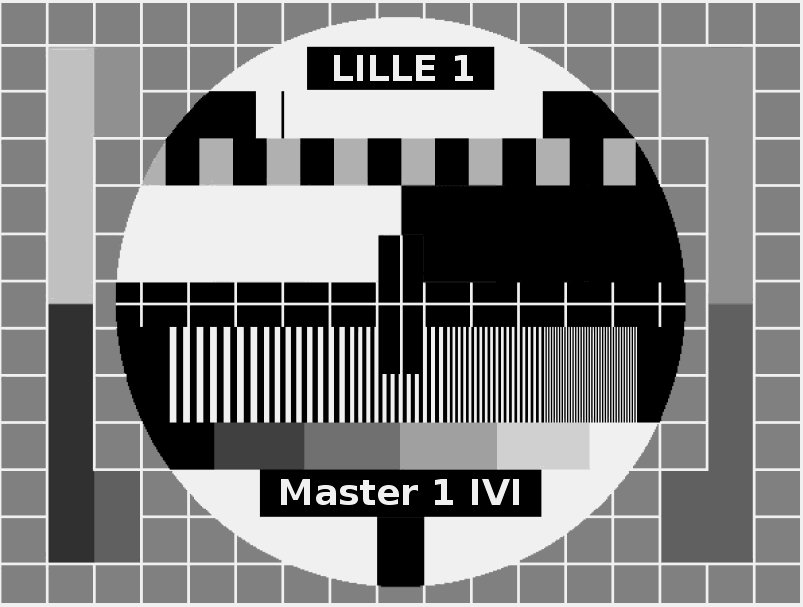
\includegraphics[scale=0.3]{image/p322.png}
	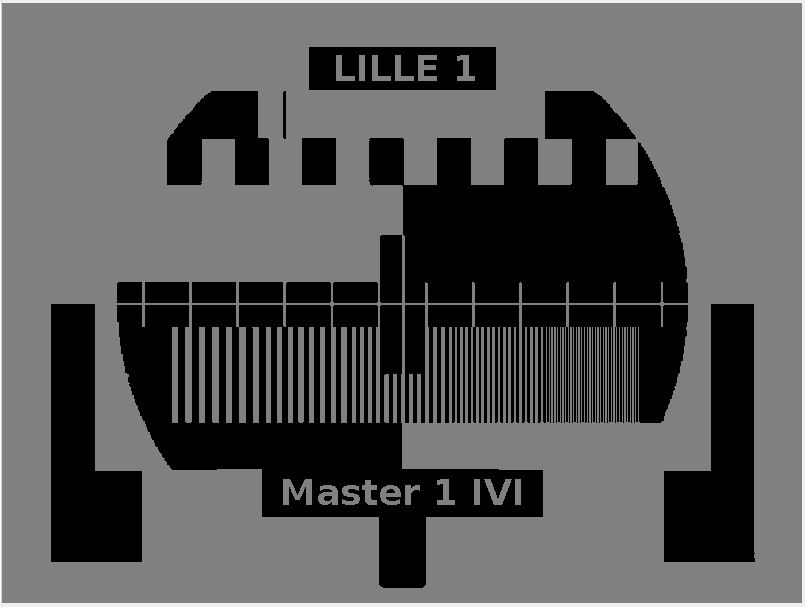
\includegraphics[scale=0.3]{image/p323.png}
\end{figure}

\noindent Voici le résultat des images, respectivement quantifiées sur 6 bits, 4 bits et 1 bits.

On constate que l'image perd en précision sur les niveaux de gris. Ce qui est normal puisque l'on passe d'un encodage 8 bits à 6, 4 et 1.

\subsection*{Utiliser les fonctions de sur et sous-échantillonnage, ainsi que la fonction de sous-quantification pour obtenir une image couleur simulant des résolutions et des quantifications différentes}


\begin{figure}[!ht]
	\center
	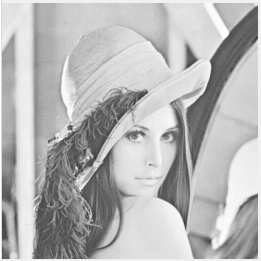
\includegraphics[scale=0.3]{image/p331.png}
	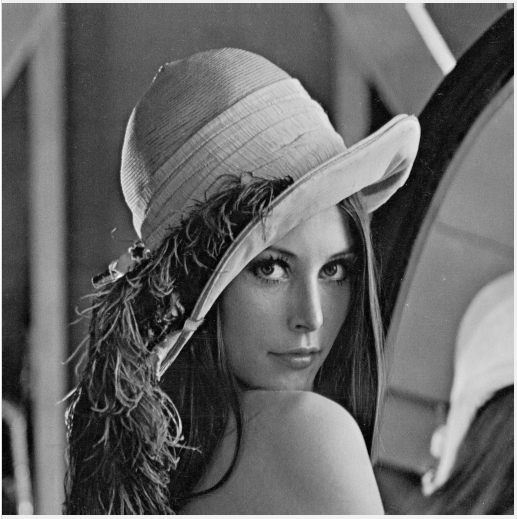
\includegraphics[scale=0.3]{image/p332.png}
	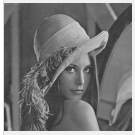
\includegraphics[scale=0.3]{image/p333.png}
\end{figure}

\noindent Voici ce que l'on obtient pour les 3 composantes demandées, respectivement composante rouge, vert, bleu.

\begin{figure}[!ht]
	\center
	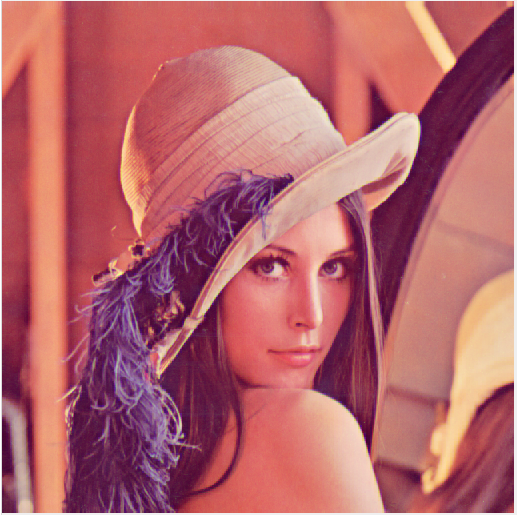
\includegraphics[scale=0.6]{image/p334.png}
	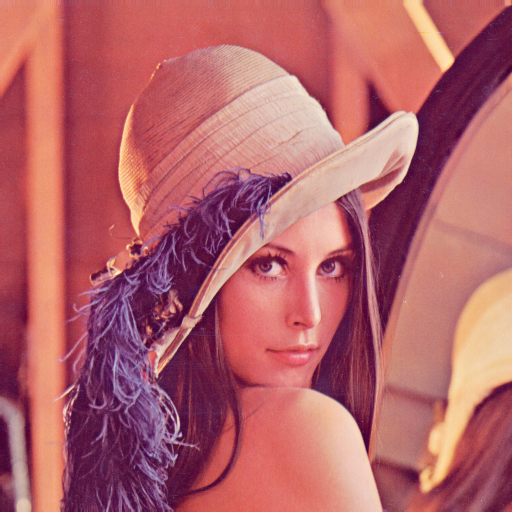
\includegraphics[scale=0.5]{../ti-semaine-3-lena.png}
\end{figure}

\noindent On obtient bien l'image de lena en additionnant les 3 composantes. Cependant on remarque que nous avons perdu (comparaison avec l'image de droite qui est l'original) en détail, une pixelisation apparaît sur l'image comme vu précédemment avec le sur-échantillonage, et nous obtenons également quelques problèmes de couleurs. Par exemple, sur les contours du chapeau du bleu/jaune apparaît, il en est de même pour les yeux, les cheuveux ...

Ce phénomène est dû au sous-échantillonage et au sur-échantillonage. Combinés sur une image couleur, il est logique que les calculs des moyennes suivi d'un sur-échantillonage perturbe la restauration d'une image couleur. Comme dit précédemment cela engendre une perte importante d'information.

\newpage
%%%%%%%%%%%%%%%%%%%%%%%%%%%%%%%%%%%%%%%%%% PART 4
%%%%%%%%%%%%%%%%%%%%%%%%%%%%%%%%%%%%%%%%%%%%%%%%%
%%%%%%%%%%%%%%%%%%%%%%%%%%%%%%%%%%%%%%%%%%%%%%%%%
\section*{Repliement de spectre}


\subsection*{Déterminer la période du motif, en pixels d'une part, et en mètres d'autre part. On considérera que la résolution horizontale est de 150 pixels/pouce. En déduire la fréquence spatiale du motif, exprimée en cycle/pixel et en cycle/m}

\noindent En observant l'image on remarque qu'il y a un motif répété 8 fois. Ce motif va d'une moitiée de bande noir à une autre, en passant par le blanc. On peut donc calculer la période $p$ du motif.\\
\begin{center}
$p$ =800/8\\
$p$=100 px \\
\end{center}

\noindent On sait qu'on a une résolution horizontale de 150px/pouce. Il  suffit de faire un produit en croix pourl'exprimer en mètres.\\
\begin{center}
150 px = 1 pouce\\
100 px = x pouces\\
x=100/150\\
x=0.66 pouces\\
x=0.016764 m \\ 
\end{center}
La fréquence spatiale du motif $f$ est égale à :
\begin{center}
$f$=1/100 px\\
$f$=1/0.016764$\sim$60 m\up{-1}\\
\end{center}


\newpage
%%%%%%%%%%%%%%%%%%%%%%%%%%%%%%%%%%%%%%%%%% CONCLU
%%%%%%%%%%%%%%%%%%%%%%%%%%%%%%%%%%%%%%%%%%%%%%%%%
%%%%%%%%%%%%%%%%%%%%%%%%%%%%%%%%%%%%%%%%%%%%%%%%%
\section*{Conclusion}

\end{document}